\chapter{Unorganized Text}

\todo{Remove this chapter}

This chapter serves as a collection of text fragments that have not yet been assigned to a particular chapter.

\section{Comparison of Existing Observability Solutions}

The list of existing observability solutions stems from \cite{9837035}.

\subsection{Evaluation Criteria}

The existing observability solutions will be evaluated by the following criteria.
\begin{enumerate}
    \item The solution covers the three pillars of observability \cite{9837035}.
    \begin{itemize}
        \item[O1]  Metrics
        \item[O2] Logs
        \item[O3] Traces
    \end{itemize}
    \item Functionality
    \begin{itemize}
        \item[F1] Correlation
        \item[F2] Topology
        \item[F3] Incident response
    \end{itemize}
    \item Characteristics
    \begin{itemize}
        \item[C1] Connected context
        \item[C2] Easier and faster exploration
        \item[C3] A single source of truth
        \item[C4] Allow capturing arbitrarily wide events
        \item[C5] Decouple data sources from sinks
    \end{itemize}
\end{enumerate}

\subsection{First Evaluation Round}

Solutions that will be picked should fulfill a majority of the above-named criteria.

\begin{longtable}{|c|c|c|c|c|c|c|c|c|c|c|c|c|}
\hline
Solution                        & O1 & O2 & O3 & F1 & F2 & F3 & C1 & C2 & C3 & C4 & C5 & Open-source \\ \hline
EMMCS                           & x  & -  & -  & -  & -  & -  & -  & -  & -  & -  & -  & -  \\ \hline
ZerOps4E                        & x  & -  & -  & -  & -  & -  & -  & -  & -  & -  & -  & -  \\ \hline
FMonE                           & x  & -  & -  & -  & -  & -  & -  & -  & -  & -  & -  & -  \\ \hline
SmartX MVF                      & x  & -  & -  & -  & -  & -  & -  & -  & -  & -  & -  & x  \\ \hline
CLAMBS                          & x  & -  & -  & -  & -  & -  & -  & -  & -  & -  & -  & -  \\ \hline
Monitoring cloud                & x  & -  & -  & -  & -  & -  & -  & -  & -  & -  & -  & -  \\ \hline
M2CPA                           & x  & -  & -  & -  & -  & -  & -  & -  & -  & -  & -  & -  \\ \hline
CL-SLAM                         & x  & -  & -  & -  & -  & -  & -  & -  & -  & -  & -  & -  \\ \hline
CloudProcMon                    & x  & -  & -  & -  & -  & -  & -  & -  & -  & -  & -  & -  \\ \hline
Self-adaptive monitoring        & x  & -  & -  & -  & -  & -  & -  & -  & -  & -  & -  & -  \\ \hline
Network-aware monitoring        & x  & -  & -  & -  & -  & -  & -  & -  & -  & -  & -  & -  \\ \hline
Monasca                         & x  & -  & -  & -  & -  & -  & -  & -  & -  & -  & -  & x  \\ \hline
Instana                         & x  & x  & x  & -  & -  & -  & -  & -  & -  & -  & -  & -  \\ \hline
Splunk                          & x  & x  & x  & -  & -  & -  & -  & -  & -  & -  & -  & -  \\ \hline
Scalyr                          & -  & x  & -  & -  & -  & -  & -  & -  & -  & -  & -  & -  \\ \hline
NetBeez                         & x  & x  & -  & -  & -  & -  & -  & -  & -  & -  & -  & -  \\ \hline
AdaM                            & x  & -  & -  & -  & -  & -  & -  & -  & -  & -  & -  & -  \\ \hline
IoT monitoring                  & x  & -  & -  & -  & -  & -  & -  & -  & -  & -  & -  & -  \\ \hline
CHARISMA                        & x  & -  & -  & -  & -  & -  & -  & -  & -  & -  & -  & -  \\ \hline
Multi-site monitoring           & x  & -  & -  & -  & -  & -  & -  & -  & -  & -  & -  & -  \\ \hline
Grafana                         & x  & x  & x  & -  & -  & -  & -  & -  & -  & -  & -  & x  \\ \hline
Kibana                          & x  & x  & -  & -  & -  & -  & -  & -  & -  & -  & -  & x  \\ \hline
Black-box Monitoring            & x  & -  & -  & -  & -  & -  & -  & -  & -  & -  & -  & x  \\ \hline
Non-intrusive techniques        & x  & x  & -  & -  & -  & -  & -  & -  & -  & -  & -  & -  \\ \hline
M3                              & x  & -  & -  & -  & -  & -  & -  & -  & -  & -  & -  & -  \\ \hline
milliScope                      & x  & x  & -  & -  & -  & -  & -  & -  & -  & -  & -  & -  \\ \hline
QoE framework                   & x  & -  & -  & -  & -  & -  & -  & -  & -  & -  & -  & -  \\ \hline
Cilium (Hubble)                 & x  & -  & -  & -  & -  & -  & -  & -  & -  & -  & -  & x  \\ \hline
ViperProbe                      & x  & -  & -  & -  & -  & -  & -  & -  & -  & -  & -  & -  \\ \hline
The rise of eBPF                & x  & -  & -  & -  & -  & -  & -  & -  & -  & -  & -  & -  \\ \hline
System visibility and security  & x  & -  & -  & -  & -  & -  & -  & -  & -  & -  & -  & x  \\ \hline
Container network observability & x  & -  & -  & -  & -  & -  & -  & -  & -  & -  & -  & -  \\ \hline
Apache SkyWalking               & x  & x  & x  & -  & -  & -  & -  & -  & -  & -  & -  & x  \\ \hline
OpenTelemetry                   & x  & x  & x  & -  & -  & -  & -  & -  & -  & -  & -  & x  \\ \hline
Consul                          & x  & x  & -  & -  & -  & -  & -  & -  & -  & -  & -  & x  \\ \hline
Prometheus                      & x  & -  & -  & -  & -  & -  & -  & -  & -  & -  & -  & x  \\ \hline
Jaeger                          & -  & -  & x  & -  & -  & -  & -  & -  & -  & -  & -  & x  \\ \hline
Dynatrace                       & x  & x  & x  & -  & -  & -  & -  & -  & -  & -  & -  & -  \\ \hline
Datadog                         & x  & x  & x  & -  & -  & -  & -  & -  & -  & -  & -  & -  \\ \hline
New Relic                       & x  & x  & x  & -  & -  & -  & -  & -  & -  & -  & -  & -  \\ \hline
Zebrium                         & x  & x  & -  & -  & -  & -  & -  & -  & -  & -  & -  & -  \\ \hline
Sumo Logic                      & x  & x  & x  & -  & -  & -  & -  & -  & -  & -  & -  & -  \\ \hline
SolarWinds                      & x  & x  & x  & -  & -  & -  & -  & -  & -  & -  & -  & -  \\ \hline
Honeycomb                       & x  & x  & x  & -  & -  & -  & -  & -  & -  & -  & -  & -  \\ \hline
\end{longtable}

\subsection{Second Evaluation Round}

Solutions
\begin{enumerate}
    \item SmartX MVF: \url{https://github.com/SmartX-Team/Visibility-SmartX-MultiView}
    \begin{enumerate}
        \item Academic Research only
        \item Specific for OF@TEIN playground on OpenStack
    \end{enumerate}
    \item Monasca: \url{https://wiki.openstack.org/wiki/Monasca/Architecture_Details#:~:text=Monasca%20is%20a%20open%2Dsource,alarm%20engine%20and%20notification%20engine.}
    \begin{enumerate}
        \item OpenStack Cloud specific
    \end{enumerate}
    \item Grafana: \url{https://grafana.com/docs/grafana/latest/introduction/?plcmt=learn-nav}
    \begin{enumerate}
        \item Visualization tool for metrics, logs and traces
    \end{enumerate}
    \item Kibana: \url{https://www.elastic.co/guide/en/welcome-to-elastic/current/getting-started-observability.html}
    \begin{enumerate}
        \item Analytics and search dashboard for Elasticsearch
        \item Part of the Elastic Stack
    \end{enumerate}
    \item Black-box Monitoring: \url{https://github.com/rolandobrondolin/DEEP-mon}
    \begin{enumerate}
        \item Data Center Power Monitoring
    \end{enumerate}
    \item Cilium: \url{https://docs.cilium.io/en/stable/overview/intro/}
    \begin{enumerate}
        \item Network monitoring and security
    \end{enumerate}
    \item System visibility and security: \url{https://github.com/samuelesabella/ebpflow}
    \begin{enumerate}
        \item Packet tracer based on eBPF
    \end{enumerate}
    \item Apache SkyWalking: \url{https://skywalking.apache.org/docs/skywalking-showcase/next/readme/}
    \begin{enumerate}
        \item Tracing, Monitoring, Logging
        \item Integrated UI
        \item Can integrate other data sources
    \end{enumerate}
    \item OpenTelemetry: \url{https://opentelemetry.io/docs/what-is-opentelemetry/}
    \begin{enumerate}
        \item Not a backend, needs a collector/storage etc
        \item Can be used to gather telemetry from basically anything
    \end{enumerate}
    \item Consul: \url{https://developer.hashicorp.com/consul/docs/connect/observability}
    \begin{enumerate}
        \item Complete service discovery etc system
        \item Supports monitoring the network
    \end{enumerate}
    \item Prometheus: \url{https://prometheus.io/docs/introduction/overview/#features}
    \begin{enumerate}
        \item Designed for mostly numeric time series data
        \item Well-known duo together with Grafana
    \end{enumerate}
    \item Jaeger: \url{https://www.jaegertracing.io/docs/1.44/features/}
    \begin{enumerate}
        \item Tracing tool by Uber: Context, Transactions, Root Cause, Topology
        \item Supports OpenTelemetry
        \item Integrated UI
    \end{enumerate}
\end{enumerate}

\subsection{Solutions Subject to Further Evaluation}

\begin{enumerate}
    \item Grafana: UI + Incident Management and different Data Sources
    \item Kibana: UI for Elasticsearch
    \item Apache SkyWalking: UI, Analytics Engine, Storage and Collection + Completely Extensible
    \item OpenTelemetry: Collection
    \item Prometheus: Analytics Engine, Storage, Collection
    \item Jaeger: UI, Analytics, Storage and Collection
\end{enumerate}

\subsubsection{Potential Combinations of Solutions}

A complete stack needs: UI, Analytics Engine, Storage and Collection

\begin{figure}[h]
	\centering
	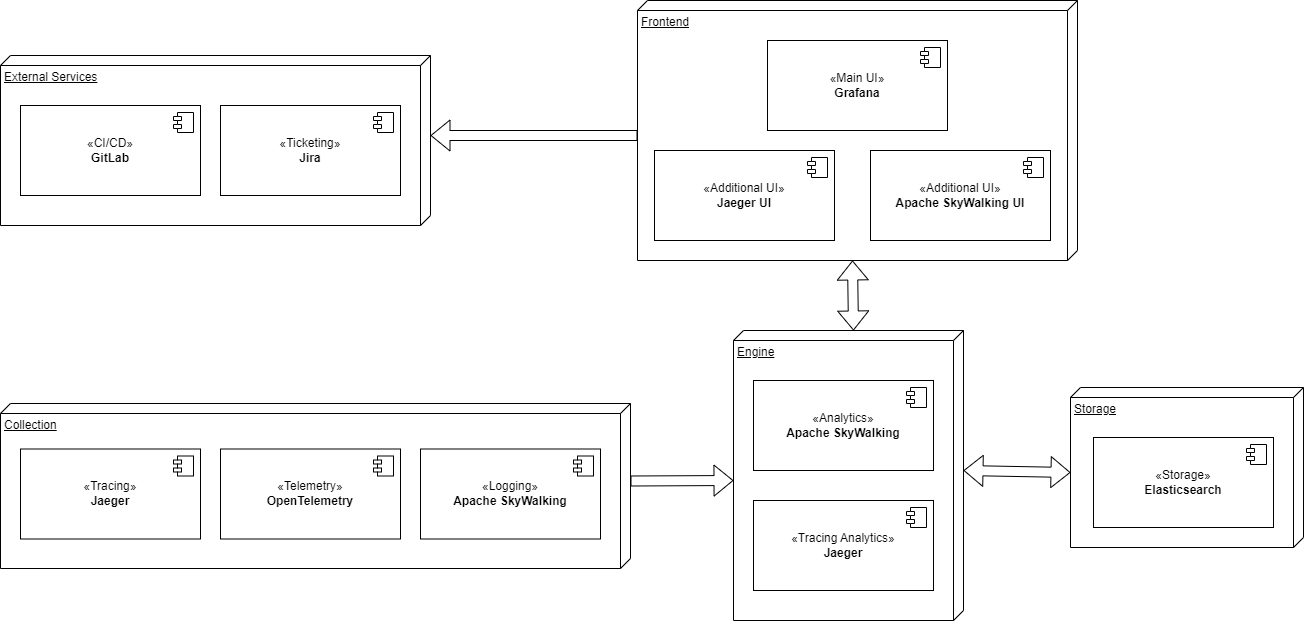
\includegraphics[width=\textwidth]{figures/ObservabilityFramework.png}
	\caption{Proposed Observability Framework}
	\label{fig:proposed_observability_framework}
\end{figure}


\subsection{Notes}

\begin{enumerate}
    \item Zipkin / OpenZipkin: network tracing for latency issues
    \item Elasticsearch: Elastic Stack search and analytics engine
    \item eBPF: Linux Kernel Observability
    \item OpenStack Cloud: PaaS
    \item Additional requirements
    \begin{enumerate}
        \item Native Helm / Kubernetes Support
        \item Open Source
        \item No vendor-specific cloud
        \item Support observing Azure VerifiedId
        \item Flexibility
    \end{enumerate} 
\end{enumerate}

